\documentclass{../../../lessonplan}
\renewcommand{\cflroot}{../../..}

\begin{document}

\lessonplantitle
    {KS1-S3}
    {Key Stage 1 Session 3}
    {Creating simple algorithms to reach a single destination}

\preamble
    {
    \item Describe the algorithm you need to reach a destination
    \item Build your code using the `direct drive' buttons
    \item Practice identifying left and right turns in a `bird's eye` view
    \item Begin to debug a sequence of instructions
    }
    {
    \item Levels 6 to 12 in Rapid Router
    \item Laptops with app or portal address bookmarked
    \item Projector or Interactive Whiteboard (IWB)
    \item Resource sheet KS1-S3-1
    }
    {
    \item Left, right
    \item Algorithm, debug
    \item Route
    }

\begin{lessonplan}

Display level 6 of Rapid Router on the IWB [fig S3.1].

\fig{fig S3.1}{figS3.1.jpg}{1}

Explain that this is a longer route that the route they were working with earlier.
The route has a few more turns so it is more of a challenge to make sure they get their lefts and rights correct.
Children will need to use the `direct drive' buttons to help them in this session.

\keyquestion{What are the first three instructions we need to start the journey to the house?}

Children can write on their whiteboards or sequence the arrow direction cards.
Choose one person to read out their sequence.

Demonstrate how to use the `direct drive' buttons to build the code.
Click on the yellow arrows and the blocks of code build up in the workspace.
The van moves with each arrow click, but once you have built up the code, you must click `Go' to get your score.
Note that in this mode, an incorrect instruction will take you `off road' and you must click `clear' to restart.

\begin{center}
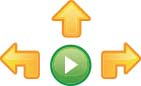
\includegraphics[width=.667\linewidth]{Arrows.jpg}
\end{center}

\keyquestion{How can we work out the distance the van travels?}
(This could be counted by the number of grid squares or sections of road you've travelled through).

Work out the total number of squares or road sections for the route.
Children can record this on their whiteboards.

\subsection*{Individual activity}

Children try levels 6 to 12.
Please note that not all children will complete each level.

Children use the app using `direct drive', or for the more advanced by dragging the blocks of code across to the workspace.

Support: some children who find left and right directions difficult may need printed versions of the route and a van card stuck onto a small cube so they can test out their instructions.

\subsection*{Share and review}

Look at level 11 together on the IWB.
Ask the children to work in pairs to write the code on the resource sheet KS1-S3-1 [fig S3.2].

\fig{fig S3.2}{figS3.2.jpg}{1}

\keyquestion{Can you count how many grid squares the route covers?}
Choose a pair of children to explain what they did.

Explain that the next time they play the app they will look at maps with more than one way to reach the house, looking for the shortest route.

The more advanced pupils may have completed level 12 and can talk about what they have learnt.

\end{lessonplan}

\end{document}
